
\chapter{Conclusiones}

FIXME

\section{Conclusiones sobre la aportaci�n de SWAML}

FIXME

\section{Trabajo relacionado}

FIXME(�la idea de swaml a que m�s podr�a aplicarse?)

\section{Conclusiones sobre Python}

FIXME

\section{Conclusiones sobre las bibliotecas utilizadas\label{sec:conclu:bib}}

FIXME(�m�s?)

\subsection{RDFLib}

RDFLib\footnote{\url{http://rdflib.net/}} FIXME

\subsection{dom.xml}

dom.xml\footnote{\url{http://docs.python.org/lib/module-xml.dom.html}} FIXME

\section{Conclusiones sobre las herramientas utilizadas}

FIXME

\subsection{Subversion}

FIXME

\subsection{Autotools}

FIXME

\subsection{Eclipse}

FIXME

\subsection{PyDev}

FIXME

\subsection{Ant}

FIXME

\subsection{SWOOP}

Existen varios editores libres para ontolog�as OWL:

\begin{itemize}
  \item Prot�g�\footnote{\url{http://protege.stanford.edu/plugins/owl/}}
  \item SWeDE\footnote{\url{http://owl-eclipse.projects.semwebcentral.org/}}
  \item SWOOP\footnote{\url{http://www.mindswap.org/2004/SWOOP/}}
\end{itemize}

Los dos primeros no son m�s que plug-ins para dar soporte a OWL en dos 
frameworks. Y el tercero es un editor pensado y desarrollado explicitamente
para trabajar con OWL.

Despu�s de las pruebas realizadas, SWOOP result� ser una herramienta m�s sencilla,
comoda de usar y potente que las otras dos.

\begin{figure}[h]
	\centering
	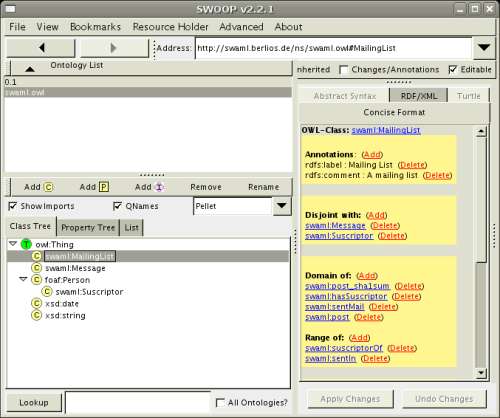
\includegraphics[width=11cm]{images/swoop.png}
	\caption{SWOOP editando la ontolog�a de SWAML en OWL DL}
	\label{fig:evoWeb}
\end{figure}

Alguna de las caracteristicas m�s interesantes de SWOOP son:

\begin{itemize}
  \item Interfaz de usuario hypermedia similar a la de un navegador convencional, 
	con elementos (pesta�as, marcadores, etc) que hacen la interfaz m�s 
	amigable.
  \item Soporte de depuraci�n de la ontolog�a.
  \item Cliente para hacer razonamientos sencillos con Pellet.
  \item FIXME
\end{itemize}

Un problema com�n en todas estas herramientas de alto nivel para trabajar con
grafos RDF es el serializado del grafo a sint�xis XML. No por su correcci�n,
que la herramienta lo hace perfectamente, sino por su orden: es muy dif�cil
que al serializar queden todos los nodos en el mismo orden. Por tanto es muy
dif�cil conocer las diferencias entre distintas versiones con las herramientas
convencionales (principalmente \texttt{diff}).

\subsection{phpWiki}

FIXME

\subsection{Google Maps}

FIXME(KML)

\subsection{\LaTeX}

\TeX/\LaTeX FIXME

\section{Lineas de futuro}

FIXME

